%Hypothese 9: Durch die Einführung der 4-Tage Woche steigt die Bereitschaft zur Weiterbildung.
%V&L

\chapter{Überprüfung der Hypothese 9}
\label{chap:hypothese9}

\section{Vorgehensweise}
Mit der Hypothese \gqq{Durch die Einführung der 4-Tage Woche steigt die Bereitschaft 
zur Weiterbildung} wird ein Fokus auf die 
Auswirkung der 4-Tage-Woche auf die Arbeitnehmenden gelegt. Auf Basis dieser Hypothese 
wurde in der Umfrage
die Frage \gqq{Würde eine 4-Tage-Woche Ihre Bereitschaft zur Weiterbildung in 
Ihrer Freizeit erhöhen?} an die Teilnehmenden gestellt.
Die Teilnehmenden konnten zwischen den Antwortmöglichkeiten \gqq{Ja}, \gqq{Eher Ja}, \gqq{Neutral}, 
\gqq{Eher Nein} und \gqq{Nein} wählen.

\paragraph*{Identifikation der relevanten Variablen}

Zu Beginn werden die unabhängigen, sowie die abhängige Variable identifiziert, welche für die 
Betrachung der Hypothese 9 relevant sind.

Die abhängige Variable beinhaltet die Daten zu der Antwort auf die Frage aus der Umfrage
\gqq{Würde eine 4-Tage-Woche Ihre Bereitschaft zur Weiterbildung in Ihrer Freizeit erhöhen?}.
Sie spiegelt direkt die Bereitschaft der Teilnehmenden zur Weiterbildung in ihrer Freizeit 
unter einer 4-Tage-Woche wider.

Für die Unabhängigen Variablen wurden die folgenden Variablen aus der Umfrage ausgewählt. 
Hier wird angenommen, dass diese Variablen einen Einfluss auf die Bereitschaft zur 
Weiterbildung der Teilnehmenden haben könnten.
\begin{itemize}
    \item Alter
    \item Geschlecht % vielleicht betrachten
    \item Kinder (Nominal)
    \item Vollzeit/Teilzeit
    % \item Führungsverantwortung
\end{itemize}


\paragraph*{Ausgewählte Analyseverfahren}

Für die Auswertung aller abgegebenen Antworten wird zuerst mit einer deskriptiven Analyse in Form eines Histogrammes
begonnen um die gesamte Meinung aller Teilnehmenden ohne Berücksichtigung der unabhängigen Variablen zu betrachten. 
Dieses ist mit einer Gaußschen Glockenkurve um den Mittelwert herum versehen, um zu betrachten, ob die Antworten 
normalverteilt sind. % warum ist das wichtig?
Hierzu werden ebenfalls der Modalwert (Modus), Median und Mittelwert der Antworten berechnet und angegeben,
um weitere Fakten über die Verteilung der Antworten zu erhalten. % Noch Standardabweichung?

Im Anschluss werden die bereits genannten unabhängigen Variablen durch Kreuztabellen betrachtet und
in passender Weise dargestellt, welche einen Einfluss auf die Bereitschaft zur Weiterbildung in der 
Freizeit unter einer 4-Tage-Woche haben könnten. 
% Für eine genauere Analyse wird eine Regressionsanalyse durchgeführt, 
% um einen tieferen Einblick in die Zusammenhänge zu erhalten. % Eventuell rausnehmen, wenn Kapitel zu lang wird


    % Auf Statistische Unabhängigkeit achten/prüfen?


\section{Analyse}

In dem folgenden Histogramm \ref{fig:bereitschaft_weiterbildung_verteilung} wird die Verteilung 
der Antworten aller Teilnehmen auf die Frage \gqq{Würde eine 4-Tage-Woche Ihre Bereitschaft 
zur Weiterbildung in Ihrer Freizeit erhöhen?} betrachtet. 

\begin{figure}[h]
    \centering
    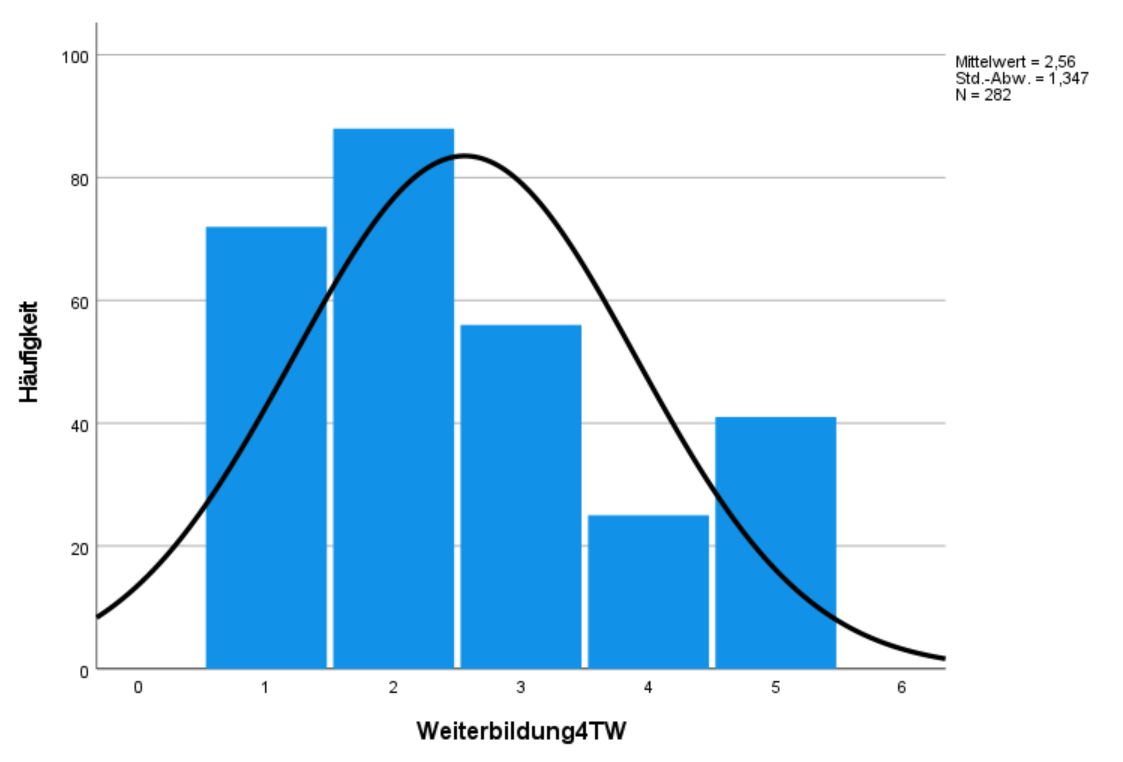
\includegraphics[width=0.7\textwidth]{04_Artefakte/01_Abbildungen/hypothese_9/histogramm_weiterbildung.png}
    \caption{Verteilung der Bereitschaft zur Weiterbildung in der Freizeit}
    \label{fig:bereitschaft_weiterbildung_verteilung}
\end{figure}

Aus dem Histogramm ist zu erkennen, dass die meisten Teilnehmenden eher 
eine Bereitschaft aufweisen sich in ihrer Freizeit weiterzubilden, 
wenn eine 4-Tage-Woche eingeführt wird.

Dies lässt ich auch anhand des Modalwertes (Modus) von 2 (Eher Ja) erkennen, welcher angibt, dass die
meisten Teilnehmenden die Bereitschaft zur Weiterbildung in ihrer Freizeit erhöhen würden.
Der Mittelwert von x und der Median von y zeigen ebenfalls auf, dass die Bereitschaft steigt.
Durch den Mittelwert ist allerdings zu erkennen, dass doch einige auch neutral oder negativ 
eingestellt sind.
% durch die Standardabweichung aufzeigen, dass die Meinung sich stärker unterscheidet?

% \begin{figure}[h]
%     \centering
%     \includegraphics[width=0.7\textwidth]{04_Artefakte/01_Abbildungen/abc.png}
%     \caption{Verteilung der Bereitschaft zur Weiterbildung in der Freizeit}
%     \label{fig:bereitschaft_weiterbildung_verteilung}
% \end{figure}

\paragraph*{Alter}

% Korrelationsanalyse machen?

\paragraph*{Geschlecht}

\paragraph*{Kinder}

\paragraph*{Vollzeit/Teilzeit}



% Korrelationskoeffizienten anschauen? Nur wenn Korrelationen zwischen den Variablen da ist,
% dann auch Regressionsanalyse durchführbar?

% 08 Teil 3

% 08 Teil 4
    % 1. Modellbildung - Notwenig? Nö, wegen SPSS?
    % 2. Berechnung der Regressionsfunktion - 2.5 (S8-97) Schrittweise?
    % 3. Test der Regressionsfunktion - Güte des Modells
    % 4. Test der Regressionskoeffizienten
    % 5. Test der Modellprämissen

\section{Ergebnis}

% Beantworten, ob die Hypothese abgelehnt oder beibehalten wird

% Annahme, da die Umfrage in dem näheren Umfeld von Personen durchgeführt wurde, die 
% Berufsbegleitend einen Master machen, kann vermutet werden, dass die Bereitschaft zur
% Weiterbildung in der Freizeit höher ist, als in der Allgemeinbevölkerung.
% Es besteht auch die Möglichkeit, dass Personen, die bereits eine Weiterbildung machen
% oder allgemein bereit sind eine Weiterbildung in ihrer Freizeit zu machen, nicht positiv 
% abgestimmt haben

% Schauen, ob die Hypothese abgelehnt oder beibehalten wird